\chapter{Produkt und Reflexion}
\section{Prozess}
\subsubsection{Erstellung der Themen Übersichten}
Nachdem der Prototyp erstellt war, wurde dieser mit den Themen Übersichten erweitert \cref{themen_uebersicht}. In die Themen Übersichten kommt man vom Homescreen und wählt danach das Unterthema aus von dem man die Informationen lesen will. 
\begin{figure}[h]
    \centering
    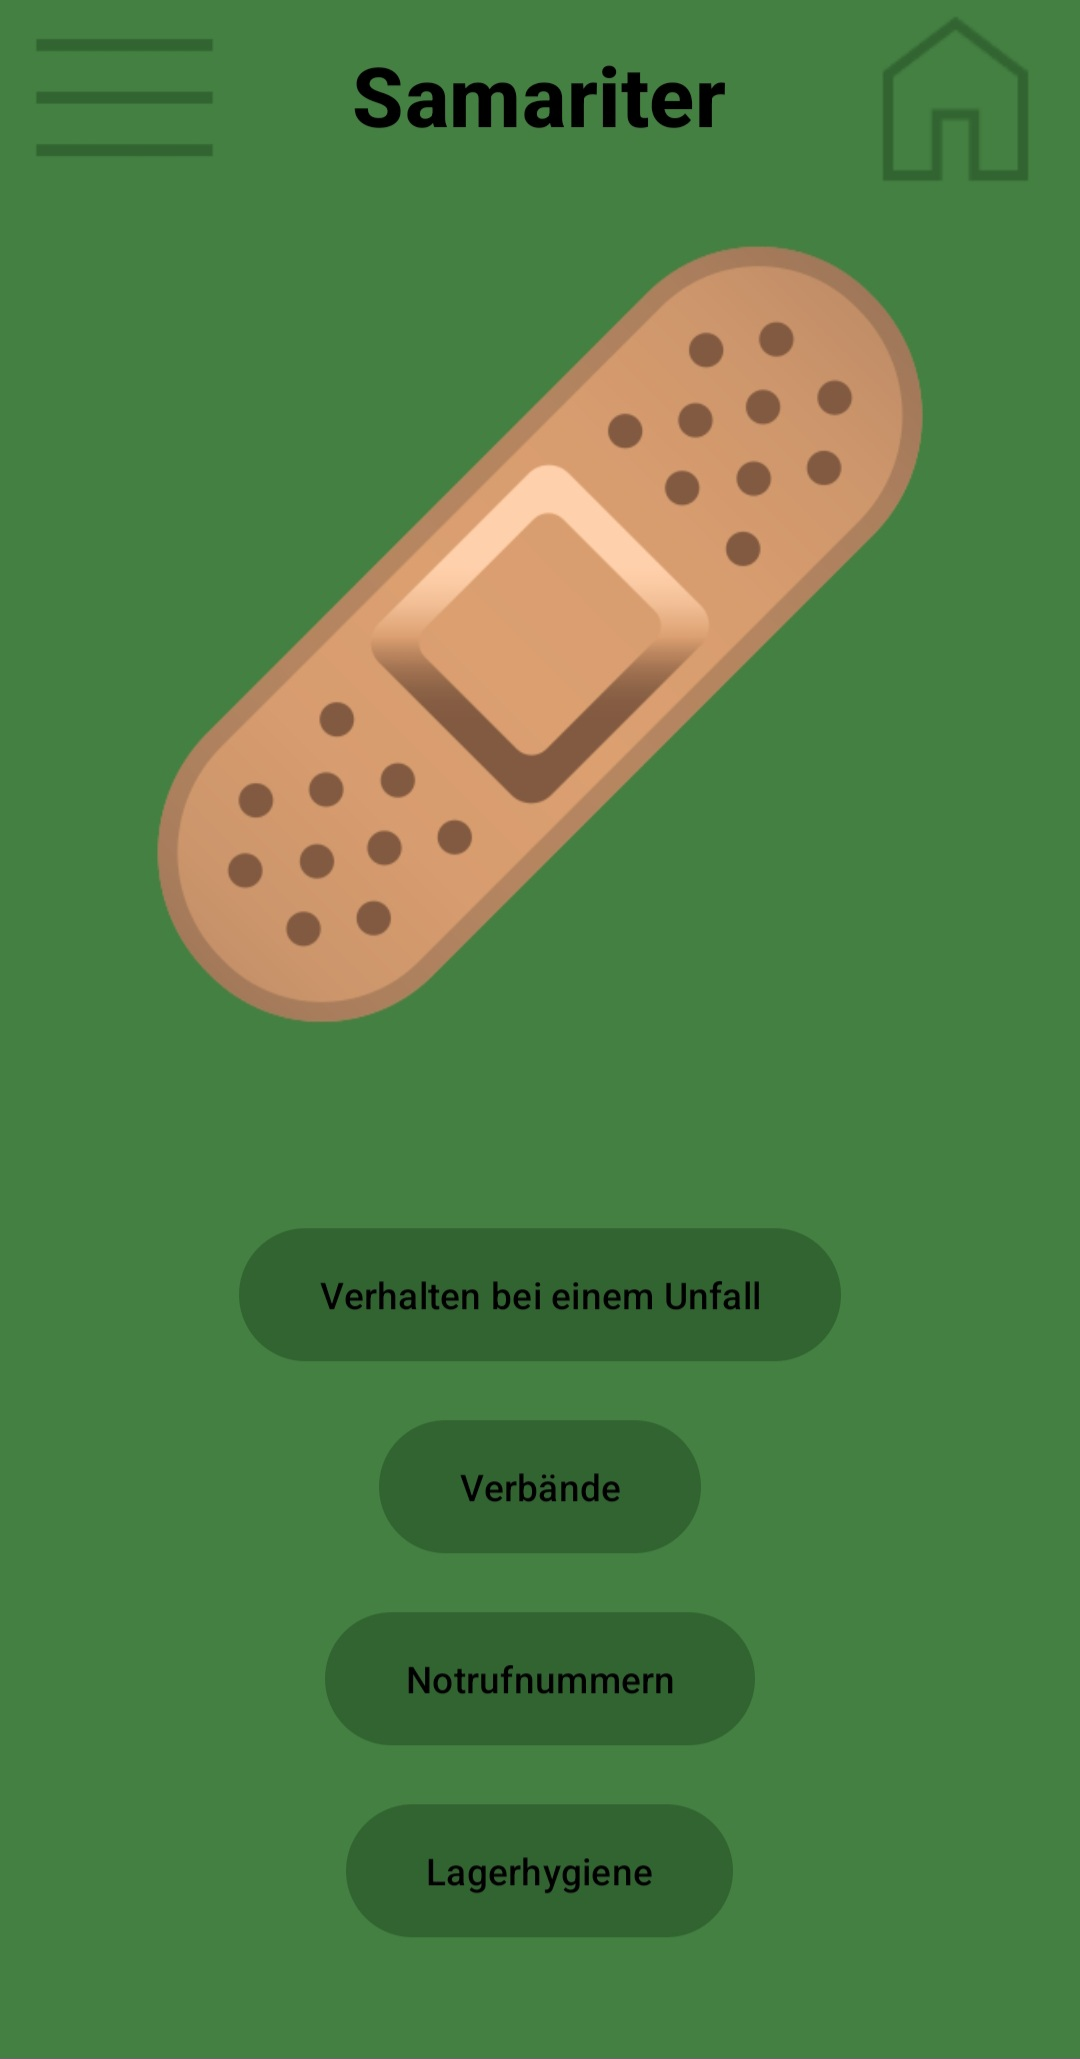
\includegraphics[width=0.33\linewidth]{Picture/themen_uebersicht.jpg}
    \caption{Themen Übersicht}
    \label{themen_uebersicht}
\end{figure}
Das Erstellen der Themen Übersichten stellte kein Problem dar, dieses kam erst mit dem Erstellen der Register der Themen Übersichten. Das Register wurde nämlich in der Aktivität des Homescreen programmiert und man kann nicht von einer Aktivität auf die andere zugreifen. \par Eine Aktivität hat immer eine eigene Layout Datei und stellt somit einen eigenen Screen dar. Auf dieser Aktivität können dann mit der Hilfe von Layouts neue Unterseiten entstehen. \par 
Um das Problem zu lösen wurde versucht eine Technik namens Fragment zu verwenden. Diese Technik ist für Sachen wie Toolbars und ähnliches entwickelt worden, zu dieser Technik wurde allerdings kein gutes Tutorial gefunden welche es ermöglicht hätte diese Technik zu verwenden. Als Lösung in jedes Unterthema das Register neu eingefügt, somit konnte das gewünschte Ergebnis erreicht werde ohne langes informieren über komplexere Techniken.\par
Nach der Lösung dieses Problemes konnten die Themen Übersichten problemlos der App hinzugefügt werden und es ging weiter mit den Informationsseiten.

\subsubsection{Erstellen der Informationsseiten}

Die Erstellung der Informationsseiten war überwiegend Fleissarbeit die erledigt werden musste, aber auch hier gab es ein kleineres Problem. Das Problem kam beim Erstellen der aktiven Notrufnummern. Das Problem hierbei war, dass man den Nutzer erfolgreich auf die Telefon App umleiten muss und das auf allen Geräten, ausserdem sollte die richtige Nummer schon eingegeben sein.\par
Um dieses Problem zu lösen wurden zwei Techniken verwendet. Die Erste war ein action dial Intent welcher der App ermöglicht, die Telefon App zu öffnen\cite{noauthor_intent_nodate}. Um nun aber noch die Telefonnummer eingetippt zu haben, muss dem Intent noch ein static URI mitgegeben werden. 
ein statischer URI \cite{noauthor_uri_nodate} dieser ermöglicht der App einen konstanten Zugriff auf die verschlüsselte Telefonnummer zu haben welche gebraucht wird für die 2. Technik. Die zweite Technik war ein action dial Intent. Ein action dial Intent ermöglicht es der App die Telefon App zu öffnen. Aufgrund des URI's der dem Intent mitgegben wird ist die Telefonnummer bereits eingegeben, wenn die App geöffnet wird.

\subsubsection{Videos}

Die letzten Probleme beim Programmieren der App kamen beim der Implementierung der Videos. Hierbei war der ursprüngliche Plan Videoviews zu verwenden da diese für Videos gemacht wurden. Diese sind allerdings sehr aufwendig zu erstellen und die App braucht dadurch deutlich mehr Speicherplatz. Die Alternative zu einer Videoview war eine Webview. Eine Webview ermöglicht es einem den Inhalt einer Website in die App zu integrieren. Diese Funktion wurde in der App so verwendet, dass ein Youtube Video in diesem Ausschnitt gezeigt wird. Diese Lösung funktioniert wunderbar bis auf den Vollbild-Button. Dieser Funktioniert aus dem Grund nicht, dass die Webview keinen Zugriff auf den gesamten Bildschirm hat und das Video somit nicht im Vollbildmodus gespielt werden kann. Dieses Problem besteht in der aktuellen Version der App immernoch.

\subsubsection{Testlauf}

Für den Testlauf war geplant, dass 3 Personen ohne Pfadierfahrung im Selbststudium mit der App sich das Wissen für die 1. Etappe aneignen. Nach einem Besuch in der Primarschule Conters hatten sich 5 Personen bereiterklärt die App zu testen. Bei der Anfangserhebung am 2.9.2024 war allerdings eine dieser Personen erkrankt und konnte nicht mitmachen. Die andern konnten den Test aber erfolgreich abschliessen. Am Ende dieser Schulwoche, fand dann die Schlusserhebung statt, die Person welche bei der Anfangserhebung krank war, war auch diesesmal nicht anwesend. Somit gab es 4 brauchbare Sets von Anfangs und Schlusserhebung. 